\chapter{多元传感信息神经隐式场景隐式重建}
从一系列RGB-D图片中进行三维表面重建是一个三维计算机视觉和计算机图形学中的基础研究问题。近年来,随着深度学习的发展,使用隐式方法,如神经辐射场\cite{mildenhall_nerf_2020},神经符号距离场\cite{wang_neus_2021}来重建隐式表面的方法取得了长足的进步,近期工作\cite{wang_neus_2021, azinovic_neural_2022}使用混合的辐射和距离场来共同表示场景的外观和几何信息。在本章中,我们对现有混合隐式场技术方案进行分析,提出这些方法中广泛存在的两种系统性误差, 这些误差会导致在使用深度信息作为监督信号时在重建的场景几何中的误差。在此基础之上,我们提出使用全方向距离场\cite{houchens_neuralodf_2022}代替符号距离场,并使用重新设计的优化方案对该隐式场进行优化可以在很大程度上消除这些系统误差对重建精度的影响。

\section{简介}
NeRF\cite{mildenhall_nerf_2020}将一个三维场景表示为一个隐式函数(如式\ref{eq:related-work radiance field}),其输入为五维坐标$(x,y,z,\theta,\phi)$,输出为RGB色值和体积渲染密度$\sigma$。对于任意一条光线$\mathbf{r}(t) = \mathbf{o} + t\cdot\mathbf{d}$上的$N$个采样点,其空间坐标被首先输入多层感知机网络来计算体密度$\sigma$,通过继续将观察角度输入后续的全连接层,可以获得该采样点的辐射颜色值。当获得了一条射线上$N$个采样点的辐射性质,我们可以用体积渲染公式(公式\ref{eq: related-work volume rendering})获得最终渲染的像素颜色值。

然而,仅通过神经辐射场的场景体积表示存在系统性的形状-辐射二义性\cite{zhang_nerf_2020}(第\ref{sec: related-work shape-radiance ambiguity}节),不能重建高质量的几何表面,因而在导出场景网格时效果较差。为了解决这一问题,现有工作主要从两方面解决这一问题。

其中一种方式是通过修改隐式场的内在结构,引入对场景几何结构更加敏感的符号距离场作为辐射场的前置组件,使用混合隐式场来构造场景表示。将符号距离场通过抽取符号距离函数$f_{SDF}(x)$的零值面来重建隐式表面。

另一种方式则是通过引入多元传感器信息输入作为额外监督信号。现有神经辐射场方法使用图片和其相机位姿作为网络输入,使用渲染颜色和真实观测颜色作为监督信号构建损失函数。通过反向传播损失函数值来优化多层感知机网络。注意到辐射场中的体积渲染方法同样可以用来计算累计深度值,为了改善该神经网络的表示精度,现有方法通过引入深度传感信息来构建额外的监督信号\cite{deng_depth-supervised_2022, roessle_dense_2022, azinovic_neural_2022}。

虽然这两种方法在一定程度上都可以弥补形状-辐射二义性,但目前的两种技术路线都不能在更大规模场景重建准确的场景几何。本文尝试将多元传感信息,特别是深度传感数据融入重建过程。然而,简单地使用深度误差优化混合隐式场存在二义性误差。在本文中,我们首先分析将这两种技术路线相结合所带来的误差。并提出基于全方向距离场的混合隐式场景表征方法。

\section{混合隐式场内在二义性}
符号距离场衡量了一个三维空间中的三维点到其最近表面的符号距离,而当符号距离函数被应用在体积渲染过程中时,通常需要显式地将距离函数值映射为体积密度或累计权重。在本文中,我们以NeuralRGB-D\cite{azinovic_neural_2022}所提出的映射方案作为示例:
\begin{equation}
    w_i = \sigma\left(\frac{f_{TSDF}(t)}{\mathtt{trunc}}\right)\cdot\sigma\left(-\frac{f_{TSDF}(t)}{\mathtt{trunc}}\right),
    \label{eq: omninerf-basedline-weighting}
\end{equation}
其中$f_{TSDF}$为神经截断符号距离函数,这个映射将符号距离函数值映射为体积积分中的点权重,$\sigma$为任意选取的钟形单峰对称函数,这里使用$\mathtt{sigmoid}$函数。这个权重分配函数在一维上的可视化如图\ref{fig:omninerf-baseline-weighting}所示。

\begin{figure}[h]
    \centering
    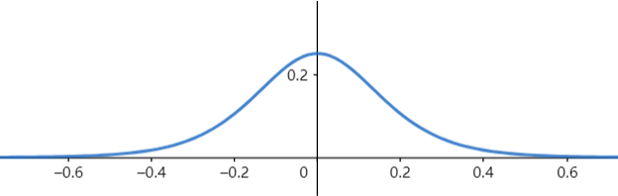
\includegraphics[width=0.6\textwidth]{undergraduate-thesis/images/neural-rgbd weighting function.png}
    \caption{公式\ref{eq: omninerf-basedline-weighting}所计算的权重函数分布。}
    \label{fig:omninerf-baseline-weighting}
\end{figure}

通过公式可以看出,距离函数较小的值将被赋予更大的体渲染权重。当距离函数通过这一函数映射到点权重后,我们可以将体积渲染公式改写为:
\begin{equation}
    \hat{C}(r) = \frac 1 {\sum_{i=0}^{N-1}w_i}\sum_{i=0}^{N-1}w_i\cdot c_i
\end{equation}

在这样的框架下, 我们描述一种由混合隐式场方案引起的系统误差。


\begin{figure}[t]
    \centering
    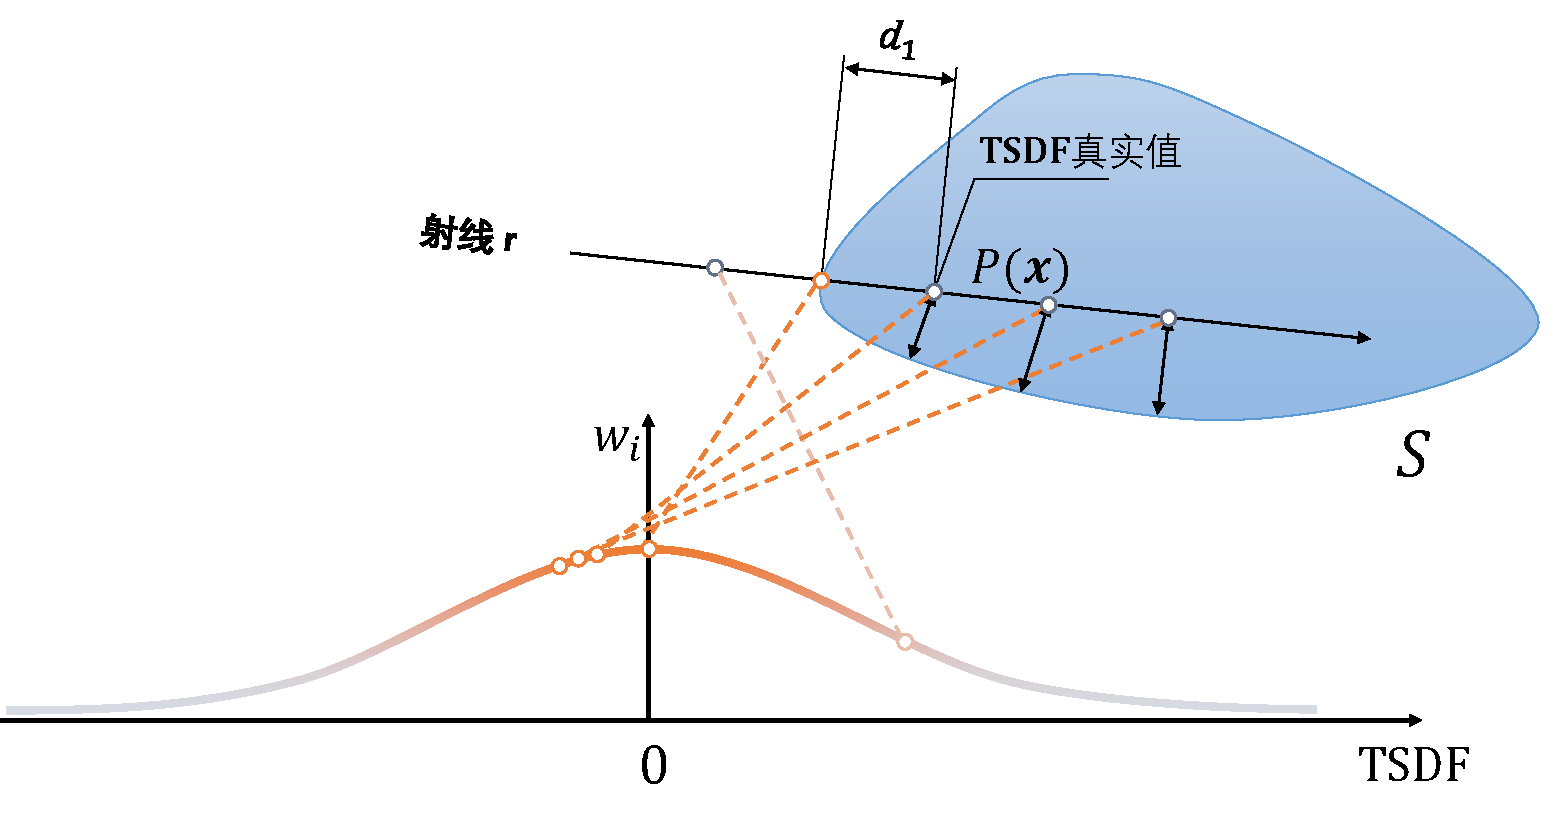
\includegraphics[width=\textwidth]{undergraduate-thesis/images/omninerf-error2.pdf}
    \caption{混合隐式场内在误差}
    \label{fig:omninerf-internal error}
\end{figure}

\section{结合深度输入的混合隐式场二义性}


\section{基于全方向距离场的混合隐式场表征}


